\documentclass[border=3mm]{standalone}

\renewcommand{\baselinestretch}{0.7}

\usepackage[usestackEOL]{stackengine}
\usepackage{xcolor}

\definecolor{palesilver}{rgb}{0.79, 0.75, 0.73}
\definecolor{silver}{rgb}{0.75, 0.75, 0.75}
\definecolor{goldenbrown}{rgb}{0.6, 0.4, 0.08}
\definecolor{glaucous}{rgb}{0.38, 0.51, 0.71}
\usepackage{tikz}
\usetikzlibrary{shapes,decorations,shadows}
 \usepackage{tikz-timing}
\usetikzlibrary{calc}
\usetikzlibrary{decorations.text}

\usepackage[siunitx]{circuitikz}


\usepackage{SevenSeg} 

\pgfkeys{
  /prob/.cd,
  angle/.initial=0,
}

%\def\object[#1](#2,#3)#4;{
%  \pgfkeys{/object/.cd,#1,angle/.get=\@angle}
%  \pgfkeys{/object/.cd,#1}
%  \node (center) at (#2,#3) {#4};
%  \coordinate (#4 center) at (center);
%  \draw [rotate around={\@angle:(center)}] ($(center)+(-1,-.5)$) coordinate (#4 a) rectangle ++(2,1);
%  \draw [rotate around={\pgfkeysvalueof{/object/angle}:(center)}] ($(center)+(-1,-.5)$) coordinate (#4 a) rectangle ++(2,1);
%  \def\@angle{0}
%}

 % probe red
%  \fill[ball color=red,shading angle=-45,rounded corners=0.2cm] (5,5) rectangle (5.4,8.5);
%  \draw[black!40,line width=0.05cm] (5.2,8.5) -- (5.2,9.1);
%  \path[color=red!50!black,line width=0.2cm] (5.2,5.5) edge [out=270 , in=0] (4.5,1.5); 
%  \path[red!50!black,line width=0.2cm,-] (4.5,1.5) edge [out=180 , in=330] (3.15,2); 


\def\prob[#1](#2,#3);{
  %\pgfkeys{/prob/.cd,#1,angle/.get=\@angle}
  \pgfkeys{/object/.cd,#1}
  \coordinate (tip) at (#2,#3);
  \fill[ball color=black,shading angle=-45,rounded  corners=0.2cm] ($(tip) - (.2,.6)$) rectangle ($(tip)+(.2,-4.5)$);
  \draw[black!40,line width=0.05cm] ($(tip)$) -- ($(tip) - (0,0.6)$);
  %\path[color=black,line width=0.2cm] (5.8,5.5) edge [out=270 , in=0] (5,1); 
  %\path[black,line width=0.2cm,-] (5,1) edge [out=180 , in=300] (2.15,2); 
}

\makeatother



\begin{document}

\tikzstyle SSGOn=[green!70!blue,line width=3pt]


\begin{tikzpicture}[even odd rule]
  
  % image
  %\node[anchor=south west,inner sep=0] (image) at (-5,0) {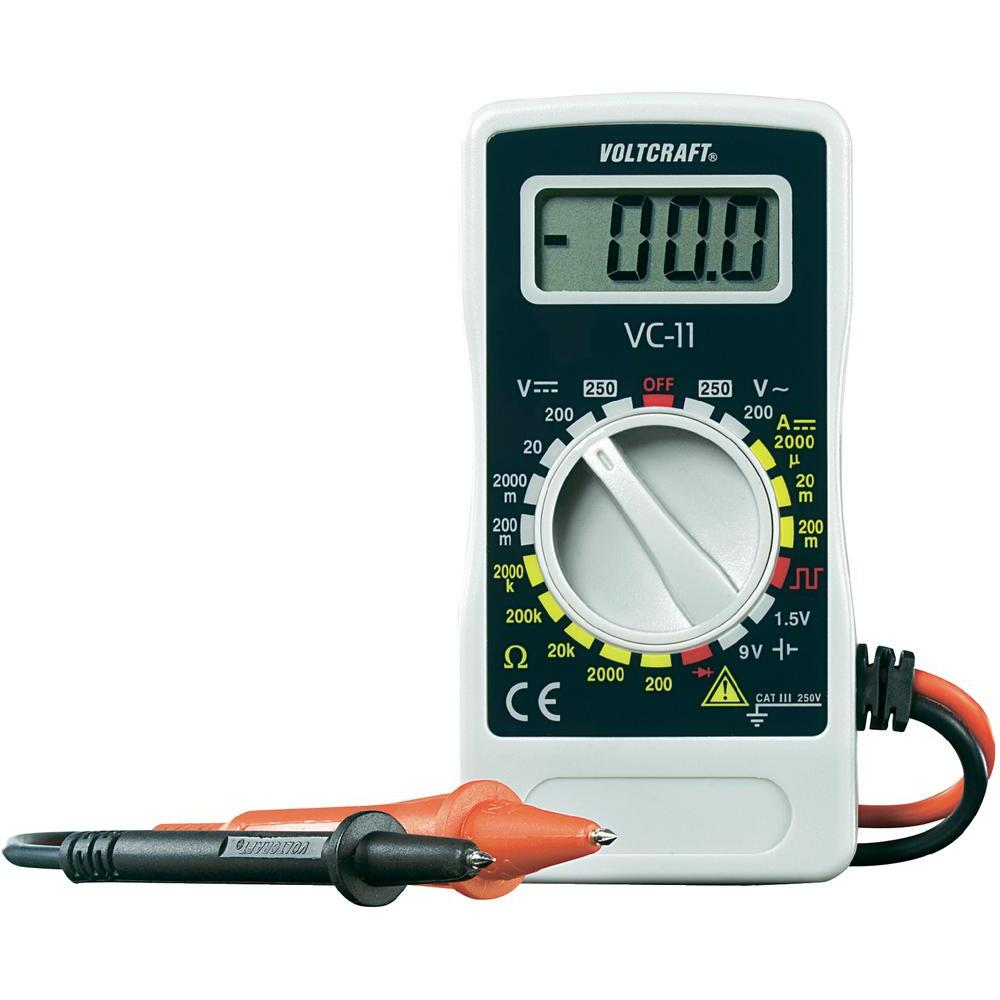
\includegraphics[width=0.9\textwidth]{multimeter-vorlage}}; 
  %\node[anchor=south west,inner sep=0] (image) at (5,0) {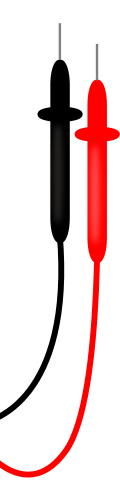
\includegraphics[width=0.2\textwidth]{kabel-vorlage}};
  % grid 
  %\draw[help lines,xstep=1,ystep=1,color=red!80] (0,0) grid (6,10);
  %\draw[help lines,thin,xstep=.5,ystep=.5] (0,0) grid (6,10);
  %\foreach \x in {0,1,...,6} { \node [anchor=north] at (\x,0) {\x}; }
  %\foreach \y in {0,1,...,10} { \node [anchor=east] at (0,\y) {\y}; } 
  % case  
  \draw[color=black!10,ball color=black!1,shading angle=-45,rounded corners=0.25cm] (0,1.35)  rectangle (4.35,9.8);
  \draw[color=black,fill=black,rounded corners=0.25cm] (0.3,2.9)  rectangle (4.05,9.5);
  % scala
  \coordinate (center) at (2.1525,5.15);
  \fill[ball color=white!80!gray,shading angle=-45] (center) circle (1.3cm);
  \fill[ball color=white,shading angle=135] ($(center)+(-0.1,-1)$) arc (-180:0:0.1) -- ($(center)+(0.2,0.95)$)  arc (0:180:0.2) --  cycle;
  \fill[ball color=black,shading angle=45] ($(center)+(-0.01,0.94)$) arc (-180:0:0.01) -- ($(center)+(0.02,1.128)$)  arc (0:180:0.02) --  cycle;
  \fill[black!30] (center) circle (1.4cm) circle (1.3cm);  
  % off
  \foreach \a/\l in {95/off} {
    	\draw[fill=red!80] ($(\a:1.4)+ (center)$) -- ($(\a:1.5cm) + (center)$) -- ($(\a-10:1.5cm) + (center)$) -- ($(\a-10:1.4)+ (center)$); 
  \node[color=red] at ($(\a-5:1.6)+ (center)$) {\tiny \l}; 
  }; 	
  % volt (AC) 		
  \foreach \a/\p/\d/\l in {113/105/1.55/250,131/122/1.55/200,149/140/1.55/20,167/160/1.53/2000\\m,185/179/1.47/200\\m} {
    \draw[fill=black!30] ($(\a:1.4)+ (center)$) -- ($(\a:1.5cm) + (center)$) -- ($(\a-10:1.5cm) + (center)$) -- ($(\a-10:1.4)+ (center)$);
    \node[color=black!30,anchor=east,align=right,inner sep=0.5ex, font=\sffamily,scale=0.5] at ($(\p:\d)+ (center)$) {\l};  	
  };
  \node[color=black!30] at ($(center) + (130:2.1)$) {V\tiny(AC)};  	
  % res.  	
  \foreach \a/\p/\d/\l in {203/199/1.5/2000\\k,221/216/1.5/200k,239/236/1.54/20k,257/257/1.6/2000,275/275/1.65/200} {
    \draw[fill=yellow!80] ($(\a:1.4)+ (center)$) -- ($(\a:1.5cm) + (center)$) -- ($(\a-10:1.5cm) + (center)$) -- ($(\a-10:1.4)+ (center)$);
  \node[color=yellow!80,anchor=east,align=right,inner sep=0.5ex, font=\sffamily,scale=0.5] at ($(\p:\d)+ (center)$) {\l};   	
  };
  \node[color=yellow!80] at ($(center) + (223:2.1)$) {$\Omega$};  	
  % diode  	
  \foreach \a/\p/\d in {293/293/8.1} {
    \draw[fill=red!80] ($(\a:1.4)+ (center)$) -- ($(\a:1.5cm) + (center)$) -- ($(\a-10:1.5cm) + (center)$) -- ($(\a-10:1.4)+ (center)$);  
    \draw[color=red!80,scale=0.2,transform shape] ($(center)+(\p-10:\d)$) to[D*] ($(center)+(\p:\d+0.4)$);
  };
  % bat  	
  \foreach \a/\p/\d/\l in {311/311/1.7/1.5,329/325/1.7/9} { 
    \draw[fill=black!30] ($(\a:1.4)+ (center)$) -- ($(\a:1.5cm) + (center)$) -- ($(\a-10:1.5cm) + (center)$) -- ($(\a-10:1.4)+ (center)$);
    \node[color=black!30,anchor=east,align=right,inner sep=0.5ex, font=\sffamily,scale=0.5] at ($(\p:\d)+ (center)$) {\l};
  };
  \draw[color=black!30,scale=0.5,transform shape,line width=0.6] ($(center)+(315:4.)$) to[battery1] ($(center)+(308:3.6)$);
  %
  \foreach \a in {347}
    	\draw[fill=red!80] ($(\a:1.4)+ (center)$) -- ($(\a:1.5cm) + (center)$) -- ($(\a-10:1.5cm) + (center)$) -- ($(\a-10:1.4)+ (center)$);
  \timing [yscale=.6,xscale=.25,color=red,timing/inline node/.style={rectangle,below left,font=\sffamily}
] at  (3.65,4.6) {L N H N L H};   	
  % ampere
  \foreach \a/\p/\d/\l in {5/0/1.5/200\\ m,23/20/1.55/20m,41/34/1.5/2000\\$\mu$} {
    \draw[fill=yellow!80] ($(\a:1.4)+ (center)$) -- ($(\a:1.5cm) + (center)$) -- ($(\a-10:1.5cm) + (center)$) -- ($(\a-10:1.4)+ (center)$);
    \node[color=yellow!80,anchor=west,align=right,inner sep=0.5ex, font=\sffamily,scale=0.5] at ($(\p:\d)+ (center)$) {\l}; 
  };  
  \node[color=yellow!80] at ($(center) + (35:2.1)$) {\small A};  	
  % volt (DC)  	
  \foreach \a/\p/\d/\l in {59/56/1.55/200,77/74/1.6/250}{
    \draw[fill=black!30] ($(\a:1.4)+ (center)$) -- ($(\a:1.5cm) + (center)$) -- ($(\a-10:1.5cm) + (center)$) -- ($(\a-10:1.4)+ (center)$);
    \node[color=black!30,anchor=west,align=right,inner sep=0.5ex, font=\sffamily,scale=0.5] at ($(\p:\d)+ (center)$) {\l}; 
  };
  \node[color=black!30] at ($(center) + (52:2.05)$) {V\tiny(DC)};  	  	  	  	  	  	 
  % LCD
  \draw[color=black!40,fill=black!5,line width=0.12cm, rounded corners=0.25cm] (0.75,7.65)  rectangle (3.6,8.95);
  \foreach \x/\l in{-1/\SSGLeg{},0/0,1/0,2/0} {
    \coordinate (L\x) at(\x*0.69+1.8,8.3);
    \SSGNb[0.4cm]{L\x}{\l}
  }
  \fill[green!70!blue] (2.8,7.9) circle(2pt);
  \fill[green!70!blue] (1,8.25) rectangle (1.25,8.37);
  % lable
  \node[color=black!30] at ($(center)+(0,4.1)$) {\small wolff-cast}; 
  \node[color=black!30] at ($(center)+(0,2.1)$) {\footnotesize m. 1}; 
  % ports
  \fill[black] (1.15,2) circle (0.28cm); 
  \fill[red!80] (1.15,2) circle (0.22cm);
  \fill[black] (1.15,2) circle (0.12cm);
  \node at (1.15,2.5) {A}; 
  \fill[black] (2.15,2) circle (0.28cm); 
  \fill[black!80] (2.15,2) circle (0.22cm);
  \fill[black] (2.15,2) circle (0.12cm);
  \node at (2.15,2.5) {COM};
  \fill[black] (3.15,2) circle (0.28cm); 
  \fill[red!80] (3.15,2) circle (0.22cm);
  \fill[red!50!black] (3.15,2) circle (0.12cm);
  \node at (3.15,2.5) {V/$\Omega$};
  % probe black
  \fill[ball color=black,shading angle=-45,rounded corners=0.2cm] (5.6,5) rectangle (6.0,8.5);
  \draw[black!40,line width=0.05cm] (5.8,8.5) -- (5.8,9.1);
  \path[color=black,line width=0.2cm] (5.8,5.5) edge [out=270 , in=0] (5,1); 
  \path[black,line width=0.2cm,-] (5,1) edge [out=180 , in=300] (2.15,2); 
  % probe red
  \fill[ball color=red,shading angle=-45,rounded corners=0.2cm] (5,5) rectangle (5.4,8.5);
  \draw[black!40,line width=0.05cm] (5.2,8.5) -- (5.2,9.1);
  \path[color=red!50!black,line width=0.2cm] (5.2,5.5) edge [out=270 , in=0] (4.5,1.5); 
  \path[red!50!black,line width=0.2cm,-] (4.5,1.5) edge [out=180 , in=330] (3.15,2); 
  
%  \prob[](7,1);
\end{tikzpicture}



%\begin{tikzpicture}
%  \object[](0,0){A};
%  \object[angle=30](3,0){B};
%  \object[](6,0){C};
%
%  \draw (A a) -- (B center);
%\end{tikzpicture}

\end{document}